\documentclass[a4paper, 12pt]{article}

% \usepackage[utf8x]{inputenc}
\usepackage[utf8]{inputenc}
\usepackage[british]{babel}

\usepackage{natbib}
\usepackage[english=american]{csquotes}

% European standard (i.e. normal space after sentence)
\frenchspacing

% Set margins to full page
\usepackage{fullpage}

% Allow doublespacing
\usepackage{setspace}

% Table rendering
\usepackage{booktabs}
\setlength{\cmidrulewidth}{\lightrulewidth}

\usepackage{graphicx}
\usepackage{caption}
\usepackage{subcaption}

% Custom labeling of description
\usepackage{enumitem}

% Add tikz for tree plotting
\usepackage{tikz}
\usetikzlibrary{positioning,fit}

\usepackage{amsmath}
\usepackage{bm} % bold math symbols
\usepackage[hidelinks]{hyperref}


\begin{document}

\setcounter{page}{0}

\title{Language as a Source of Misclassification in the Human Coding of Political Texts\footnote{We thank Ken Benoit and Ben Lauderdale for helpful comments and discussions on this project. Naturally, errors remain our responsibility.}}
\author{
  Tom Paskhalis\\ \textit{\small London School of Economics} \\ \href{mailto:t.g.paskhalis@lse.ac.uk}{\ttfamily\small t.g.paskhalis@lse.ac.uk}
  \and
  Christian Mueller\\ \textit{\small London School of Economics} \\ \href{mailto:c.mueller@lse.ac.uk}{\ttfamily\small c.mueller@lse.ac.uk}
}


\maketitle
\thispagestyle{empty}

\vspace{3em}

\begin{abstract}
\noindent Designing valid and reliable method for coding large quantities of text is an inherently complicated process. Manual text coding of political manifestos has been shown to be prone to a range of problems that can lead to unreliable results. These include complex coding scheme, intransparent unitization and lack of uncertainty estimates that stem from using only one coder per manifesto. However, the linguistic features that can account for coding errors and the implications of ignoring them have not yet been studied yet. A considerable body of literature in psycholinguistics shows that certain types of sentences are more difficult for humans to process. For example, negative sentences, on average, are harder than their affirmative equivalents. Sentences with main and subordinate clauses appearing in a reversed order might also result in more coding errors. At the same time, current text-as-data approaches work around this limitation of mental syntactic parsing by entirely disregarding word order. In this paper we investigate the effects of negation and main clause position on manual annotation of sentences from party manifestos by crowd-sourced workers. Our results show that both of these features appear to affect coders' ability to discriminate between policy positions. We argue that for measurement models where the theoretical construct can be expected to manifest itself in word frequencies, automated methods outperform humans due to the way language operates.
\end{abstract}

\clearpage
% \setcounter{page}{1}
\doublespacing

\section{Introduction}

Political scientists have long been using content analysis to study texts produced by political actors. Since the original works of \citet{Berelson1948} and \citet{Lasswell1949}, researchers turned to systematic reading and coding of texts by human subjects to make inferences about their analytical constructs. Despite the recent advances in computerised text analysis \citep{Grimmer2013}, manual coding remains extremely common technique among applied researchers. The reasons for that are three-fold. First, some analytical constructs accessible to human readers, could still be elusive for machines and, thus, cannot be readily outsourced to computers. E.g. deliberation, conceived as participatory and inclusive debate where rational arguments of all sides can be expressed and considered in a respectful manner, which has generated a large body of both empirical \citep{Fishkin2005, Steenbergen2003} and theoretical literature \citep{Dryzek2004, Gutmann2004}, has so far been studied exclusively with manual quantitative and qualitative content analysis. Second, although in principle some uses of human coders can be automated, in practice the associated costs might end up being equal or higher than employing research assistants. Named entity recognition and labelling, while being a highly promising technique in natural language processing, requires a large quantity of tailored training data, manually annotated by human coders. The latter can defeat the original purpose of reducing the costs and making research less prone to subjective decisions. And, finally, while using text as their primary source of data and human coding as a chief method of inquiry, certain analytical frameworks can assume that the inferences depend not exclusively on the content, but on a broader political and societal context that has to be taken into account. While some or all these arguments can be germane to a particular subject and topic, quantitative text analysis has been shown to be a valid, reliable and replicable method for estimating party \citep{Laver2003, Slapin2008}, legislators' \citep{Lauderdale2016} and interest group \citep{Kluver2009} positions, helping predict electoral results \citep{Beauchamp2017} and disentangling the mechanisms of state censorship \citep{King2013}.

The methodological advancement in estimating quantities of interest from textual data has not been met, however, by a theoretical understanding of the processes that allow them to perform so well. Considering the predominant \enquote{bag-of-words} model, that underpins the absolute majority of new methods, most researchers admit that the key assumption made by the model that word order does not matter and can be ignored without losing much information does not reflect how language works. Even more unrealistic assumptions are made by so-called \enquote{topic models} \citep{Blei2003} that posit that every word comes from a distribution of topics. Thus, several words appearing sequentially in a single sentence can come from multiple topics. A rather non-trivial presumption given our knowledge of linguistics and everyday speech experience. One of potential explanations could be that these modelling simplifications, while counter-intuitive from a linguistic point of view, in practice avoid the pitfalls that human coders might fall into. Although more consistent with our understanding of language, taking text units as a whole inevitably incorporates their ambiguities and complexities. We argue that in cases where the quantity of interest can realistically be assumed to be expressed in word frequencies, automated methods of text analysis can be as accurate or even outperform humans due to the way language operates. Empirically, in this study we test our proposition on Manifesto Project, the largest project in the analysis of political text. Most importantly for our purposes, multiple methods, both involving human coders and automated text analysis have been shown to produce reasonably accurate estimates of party policy positions and their shifts over time.

\section{Content Analysis Overview}
We start with a brief overview of content analysis. Following \citet{Krippendorff2004}, who offers the most comprehensive treatment of the method, content analysis can be divided into 6 steps. (1) \textit{Data collection}, the initial stage of most research, in the case of content analysis involves gathering the texts that are anticipated to contain the information that can answer researcher's question. With the rise of internet and large-scale projects on digitalisation of paper-based documents, the range of potential sources can vary widely, from newspaper articles to parliamentary speeches to messages on social media. (2) \textit{Unitization} is an important decision of how to divide the collected data into individual units that are then analysed. Typical examples would be entire text, paragraph, sentence and word. The latter being an implied unit in many automated methods of analysis, that can then be aggregated at a higher level of sentence or text. (3) \textit{Sampling} gets far less attention in typical applications of content analysis than it deserves. This puts content analysis in sharp contrast to many other quantitative methods, such as surveys or experiments, where sampling is considered a crucial step in generating valid and reliable estimates of the phenomenon of interest. While conceptually the population of texts to which a researcher makes an inference is a more elusive notion than survey population (Does it encompass all the produced texts that are of interest? Or only recorded? Or even those that could have been generated but were not for various reasons?), we believe it is an important procedure for a carefully designed research that involves content analysis. (4) The \textit{application of analytical framework} roughly corresponds to what Krippendorff calls recording and reducing. In the case of manual human coding this involves getting and training coders, which in a simpler case might mean familiarising them with the codebook and in a more complicated in-depth instruction about the concepts of interest. Subsequently, they are given the texts sampled at the previous step to apply the labels in accordance with the coding instructions. For computerised text analysis at this step the researcher prepares the sampled corpus by putting them in a format required by specific software used for the analysis\footnote{This step can include stemming and removing stopwords, the terms that are deemed irrelevant for the analysis.} and then runs the analysis. It is this step that will be the primary focus of our study, as here manual content analysis and automated methods begin to diverge and it is the starting point of much of the discrepancies in the final results. After applying a chosen framework, the method generates some quantities that can then be used to (5) \textit{make inferences} about the studied phenomenon. It is often the case that how inferences are made is, at least, partially determined by the framework. In some cases it could be a word frequency cross-tabulation, in others it would be coefficient estimates from a hierarchical model. (6) And, finally, after interpreting the estimates, researcher \textit{narrates} the results by connecting them back to the literature, context and research question.

The core steps of content analysis (2-4), described above, all treat some segment of text as a unit of analysis. While most automated methods operate on what is called document-term matrix, where rows represent documents and columns record the number of times a given word occurs in that document. Most importantly, the order of rows and columns in the matrix is arbitrary. This drastically contrasts with human coding in that the segments must retain structure to make it possible for humans to read and interpret them. To give a concrete example, the sentence: \enquote{We will not cut benefits.} has to be presented to a human coder intact, while a computer can equivalently read a vector of words: \enquote{benefits}, \enquote{cut}, \enquote{not},  \enquote{we}, \enquote{will}, where the last three terms are likely to be removed as stopwords. Although, superficially, it might seem that the former contains more information, we argue that this is, ultimately dependent on the type of the quantity of interest. In other words, notions, such as saliency that are likely to be expressed in the repetition of some terms or their combinations, are equally accessible to machines, as opposed to more nuanced concepts such as valence of deliberation. The intuition behind it is that by potentially treating texts more coarsely than human coders, automated methods avoid some of the difficulties inherent to language.

\section{Psycholinguistic Foundations}
In this study we are focussing on sentence as a unit of analysis. In the context of coding party platforms from their manifestos quasi-sentence has long been a unit choice \citep{Volkens2013}. Quasi-sentences as opposed to natural sentences allow for the possibility that a single sentence contains several policy propositions that can span multiple codes or even policy domains. Although not unlikely given the language complexity of some party programmes, this has been shown to be prone to arbitrary decisions made by coders while producing no appreciable differences in substantive conclusions \citep{Daubler2012}. Recently, there has been also some progress in political science in grounding this choice not only on the basis of methodological considerations, but also on linguistic theory \citep{Dolezal2016a}.

The choice of a unit of analysis is tightly linked to the psycholinguistic origins of our central hypothesis. Since the seminal work of \citet{Chomsky1957}, sentence re-emerged as a primary building block of language and unit of perception\footnote{Although sentence generated considerable interest among the founding figures of psychology, such as Wilhelm Wundt and William James, it fell into disrepute with the rise of behaviourism. For a comprehensive historical overview see \citet{Townsend2001}.} Chomsky's theory of transformational grammar described sentence as a syntactic configuration generated from kernels by a set of phrase structure rules that constituted the syntax of language. Knowing or learning language in this view, essentially, means possessing or acquiring these rules that allow to distinguish sentences from non-sentences. The idea that not all sentences are created equal followed soon after this theoretical breakthrough. In his landmark article, \citep{Miller1962} defined eight types of sentences formed by three possible transformations of the kernel (K) sentence and their combinations: negative (N), passive (P), interrogative (Q), negative passive (NP), negative interrogative (NQ), passive interrogative (PQ) and passive negative interrogative (PNQ).

\begin{figure}[!htb]
\begin{minipage}{0.4\textwidth}
\centering
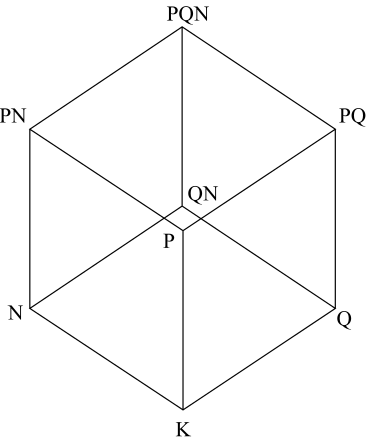
\includegraphics[width=0.8\linewidth]{sentence_cube.png}
\subcaption{}
\label{fig:sub:sentence-cube}
\end{minipage}
\begin{minipage}{0.6\textwidth}
\centering
\vspace{0.5cm}
\footnotesize
\begin{description}[font={\footnotesize}]
\item [K] Conservatives will introduce means testing.
\item [N] Conservatives will not introduce means testing.
\item [P] Means testing will be introduced by Conservatives.
\item [Q] Will Conservatives introduce means testing?
\item [NP] Means testing will not be introduced by Conservatives.
\item [NQ] Won't Conservatives introduce means testing?
\item [PQ] Will means testing be introduced by Conservatives?
\item [PNQ] Won't means testing be introduced by Conservatives?
\end{description}
\vspace{0.5cm}
\subcaption{}
\label{fig:sub:sentence-example}
\end{minipage}
\caption{Sentence transformation cube \citet[adapted from figure~12 on p.~760]{Miller1962} (a) and a manifesto-type example of its application (b).}
\label{fig:sentence-figure}
\end{figure}

Figure \ref{fig:sentence-figure} shows the relationships between all of the eight types by positioning them on the edges of a three-dimensional cube. The crucial insight, confirmed by a number of experimental studies \citep{Gough1965, Mehler1963} was that the time required to form or process a sentence given another variant of it is a function of their proximity on the cube. Some of the sentence forms, e.g. passive negative interrogative (PNQ) are rather uncommon in written political texts\footnote{This, however, might not necessarily apply to speeches.}. Other variants, especially the negative, can be expected to occur more frequently. In addition to transformations of simple sentence structure, composite sentences, formed of several clauses, add another layer of complexity. For example, \citet{Holmes1973} has shown that the order of main and subordinate clauses can equally affect sentence perception. Given the structure of many party programmes and the involvement of humans in parsing and coding sentences, we would expect these cognitive phenomena to affect the resultant estimates. In this study we focus particularly on two syntactic structures most likely to arise in party manifestos: negation and change of sub-clause position.

\section{Model of Text Classification}
Current approaches to text misclassification tend to focus on the coding scheme and coding instructions that can affect the reliability of estimates \citep{Krippendorff2004}. In effect, these models posit that by crafting a more balanced and intuitive coding scheme, coupled with clear instructions, researchers can improve the reliability of manually tagging text units.

\citet{Mikhaylov2012} provide the most comprehensive treatment of stochastic misclassification of text units. In this framework misclassification happens through a process described by the following equation
\begin{equation*}
  P(T^*_i = j\,|\,T_i = k) = \theta_{jk},
\end{equation*}
where $j, k = 1, ..., m$ is a code assigned to each text unit out of $m$ categories defined by the coding scheme. $\theta_{jk}$ is an off-diagonal cell in the $m \times m$ matrix $\bm{\Theta}$ that represents text units that were coded as $j$, given their true label $k$. Perfect coding would imply that matrix $\bm{\Theta}$ is a diagonal matrix. Insofar that no real coding is ideal, this matrix would contain off-diagonal elements that result in biased estimates of $T_i$.

Rewriting the model above as a data-generating process, a text units $T_i$ can be assumed to follow a multinomial distribution
\begin{equation*}
  T_i \sim \operatorname{Multinomial}(n, \bm{p}),
\end{equation*}
where $\bm{p}$ is a vector of parameters over $m$ categories, specified by the codebook. Here the typical goal is to find the population parameters $\bm{p}$\footnote{Assuming $\bm{\Theta}$ is a diagonal matrix, the vector of interest $\bm{p}$ can be expressed as $\bm{p} = (\frac{\theta_{\cdot 1}}{\theta_{\cdot\cdot}}, ..., \frac{\theta_{\cdot m}}{\theta_{\cdot\cdot}})$} that can be thought as the probabilities for individual text units of coming from a certain category or, equivalently, the proportions of the whole text truly belonging to each category. By manipulating the number and the content of codes, researcher implicitly changes the parameter vector $\bm{p}$, which can assume different forms. While being mostly theory-driven, certain forms can be more difficult to estimate in practice. More uniform parameter vector, such as $\bm{p}_3 = (0.3, 0.3, 0.4)$ can be easier to estimate given the same amount of data than $\bm{p}_3 = (0.05, 0.05, 0.9)$. Although without applying the scheme, it is hard to know what population parameters are, we can assume that an increase in the number of codes will lead to a larger number of categories with very small probabilities, which can result in imprecise estimates. We alleviate this problem by relying on a simplified version of 56-category coding scheme used in Manifesto Project \citep{Volkens2013}, that was adopted by \citet{Benoit2016}.

Another implicit assumption of this model of text classification is that each text unit has identical parameter vector. However, linguistic and stylistic choices can affect the probabilities of individual text units truly belonging to a certain category. As discussed above, it is not unreasonable to anticipate heterogeneous error due to ambiguity in the sentence. More formally, the vector of probabilities $\bm{p}$, rather than being a fixed quantity, might itself come from a distribution
\begin{equation*}
  T_i \sim \operatorname{Multinomial}(n, \bm{p}_i).
\end{equation*}
Adding another level to the text classification model allows us to reason about the coding process not only in terms of a pre-adopted scheme, but also in terms of linguistic variation that can drive the choice of a specific code. Rather than estimating $\bm{p}_i$ directly, in the empirical part we are focussing on the effects of negation and sub-clause position on the sentence-level ambiguity that, in turn, can bias the estimates of the quantity of interest if not properly accounted for.

\section{Data}

The key requirement to be able to assess how language itself might make certain text units more prone to coding errors is that each text unit was coded multiple times by different coders. This requirement is not easy to satisfy with the currently available data as most empirical studies rely on one or, at best, a handful of coders \citep[e.g.][]{VLM+2016,Dolezal2016a}. Although it allows to calculate intercoder reliability on an aggregate level of text, it does not permit the granularity that our hypothesis assumes. In order to test our hypothesis about the effects of linguistic features on misclassification rate, we use the data generated by the crowd-sourced coding of party manifestos in Britain \citep{Benoit2016}. By definition, crowd-source tasks assumes that many readers code multiple text units at least several times. Thus, making this data source come closest to the ideal experimental scenario, where actual sentences could be manipulated.

In order to test for whether there are certain linguistic features which certain misclassifications can be attributed to, we use texts from the most coded corpus of political texts, the Manifesto Corpus \citep{MRL2016-04} and the efforts in the Manifesto Project \citep{VLM+2016} more generally. It is the longest, most consistent effort in human coding of political text and provides a good testing ground for the hypothesis. Furthermore, several automated methods have been developed over time for extracting ideological positions and identifying positional shifts between elections \citep{Laver2003, Slapin2008, Lo2016}. When considered together, these studies provide substantial evidence that ideological position can be reliably estimated with models based on \enquote{bag-of-words} assumption that word order can safely be disregarded.  Unfortunately, the Manifesto Project dataset only contains codings from a single coder \citep{Mikhaylov2012}. This makes it impossible to estimate sentence-level ambiguity parameter and control for coder-specific effects. In order to account for those effects, we rely on a data set of codings of sentences taken from 18 British party manifestos between 1987 and 2010 coded by a small number of expert coders and a large number of crowd workers collected by \citet{Benoit2016}.

\begin{figure}[htpb]
  \centering
  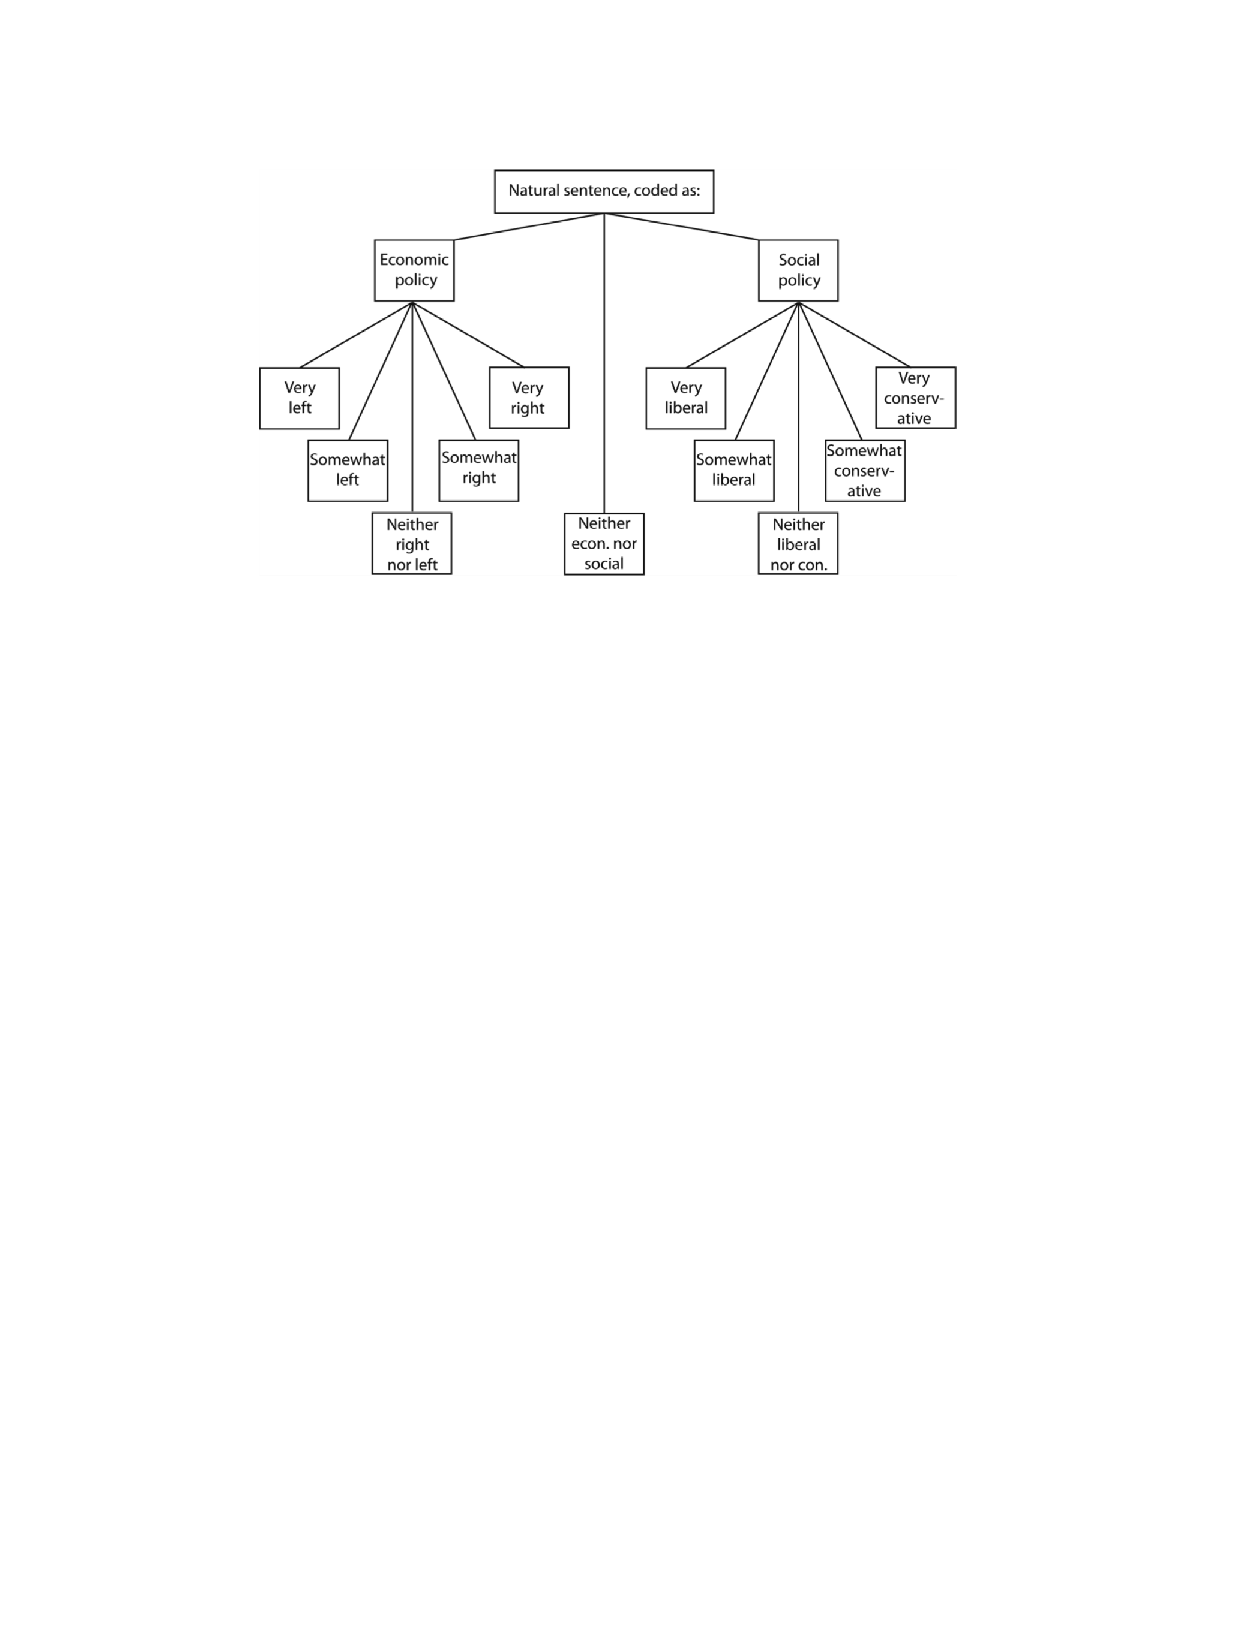
\includegraphics[width=0.8\linewidth]{coding-scheme-benoitetal.pdf}
  \caption{Simplified coding scheme used by \citet[taken from figure~1 on p.~281]{Benoit2016}.}
  \label{fig:coding-scheme}
\end{figure}

In these data, coders were individual sentences and they had to code them according to the simplified two-part coding scheme in figure~\ref{fig:coding-scheme}. The first part of the task was to decide whether a sentence contains statements related to economic or social policy. If the policy domain was determined to be either economic or social, the sentence had to be coded on a five-point ordinal scale ranging from \enquote{very left} to \enquote{very right} and \enquote{very liberal} to \enquote{very conservative} for the economic and social dimensions respectively.

\begin{table}[htbp]
  \centering
  \begin{tabular}{lrrrrrrr}
    \toprule
    Level & Min. & 1st Quart. & Median & Mean & 3rd Quart. & Max. \\
    \midrule
    Coder & 3 & 10 & 14 & 144 & 69 & 10180 \\
    Sentence & 4 & 5 & 5 & 10 & 15 & 215 \\
    \bottomrule
  \end{tabular}
  \caption{Coder- and sentence-level summary statistics of number of codings.}
  \label{tab:summary-codings}
\end{table}

It is plausible, however, that even a limited subset of sentence transformations does not occur often enough in party programmes to make a difference for human coding. Table~\ref{tab:summary-linguistic} shows the percentages of sentences in British party manifestos. These percentages are not only non-trivial, ranging from 4\% to 10\% of all sentences for negation and from 4\% to 14\% for prepositional phrases, they also covary with changes in electoral politics. We can observe a lagged increase in the number of negative sentences when a party switches from ruling to opposition status and vice versa. Conservatives in their 2001 manifesto after landslide victory by Labour in the previous election, used 3 percentage points more negative sentences in their manifesto than in 1997. This spike tails off, but never goes back to pre-1997 level. Labour, on the contrary, reduce their proportion of sentences containing negation from 10\% to 5\% between 1997 and 2001. The implications of this association between linguistic features and politically relevant phenomena are two-fold. First, when relying on human readers to code sentences, the texts have to be either tested for their linguistic heterogeneity prior to commencement of coding\footnote{The emerging literature on linguistic complexity can provide one avenue for such testing \citep{Spirling2015}.} or these differences have to be modelled explicitly. Second, when not accounted for this differential usage of certain linguistic features can not only bias the estimates, but do so in a way that is hard to predict.

For the main analysis, we focus on the coding decision of the crowd workers and exclude the codings by expert coders. These data contain 184,328 coding decision for 18,263 sentences made by 1,280 crowd workers. Table~\ref{tab:summary-codings} contains summary statistics of the number of codings in our the data by coder and sentence. The median, which provides a good estimate for the average number of codings because the distribution of both variables is highly skewed, for coders is 14 codings and for sentences is 5 codings. Thus, each sentence has been coded on average by 5 different coders, each of whom coded on average 14 sentences.

We identify and incorporate three different language features with a potential for effecting misclassification.\footnote{We rely on \texttt{spacy}, a natural language processing framework in Python, to do the part-of-speech tagging and dependency parsing. See \citet{CTS2015} for an evaluation of the crucial dependency parsing component.} The first potential source for misclassification is negation as negated statements, e.g. saying \enquote{we do not support} instead of \enquote{we are against}, tend to be harder to comprehend than their affirmative equivalents. We automatically extract an indicator for whether the sentence contains negation from the parsed text by looking for dependency relations of type \enquote{negation modifier} \citep[see][33]{CP2012}.

\begin{table}[htpb]
  \centering
  \begin{tabular}{lrrrrrr}
    \toprule
    & & Sentence & Words & Negation & Prepositional & Subclause \\
    Party & Year & \multicolumn{1}{c}{(N)} & \multicolumn{1}{c}{(avg.)} & \multicolumn{1}{c}{(\%)} & \multicolumn{1}{c}{(\%)} & \multicolumn{1}{c}{(\%)} \\
    % \cmidrule(lr){1-2} \cmidrule(lr){3-6}
    \midrule
    Conservatives & 1987 & 1015 & 17.5 & 6.5 & 11.4 & 18.9 \\
    Conservatives & 1992 & 1731 & 17.1 & 4.9 & 12.6 & 21.8 \\
    Conservatives & 1997 & 1171 & 17.9 & 7.4 & 10.8 & 18.4 \\
    Conservatives & 2001 & 748 & 16.9 & 10.0 & 8.0 & 21.4 \\
    Conservatives & 2005 & 414 & 17.0 & 7.5 & 12.8 & 26.6 \\
    Conservatives & 2010 & 1240 & 20.6 & 8.2 & 9.3 & 35.6 \\
    \addlinespace
    Labour & 1987 & 455 & 20.0 & 5.1 & 9.7 & 19.6 \\
    Labour & 1992 & 661 & 18.7 & 5.0 & 12.0 & 28.4 \\
    Labour & 1997 & 1052 & 16.6 & 10.3 & 7.6 & 19.6 \\
    Labour & 2001 & 1752 & 17.2 & 5.3 & 9.2 & 25.8 \\
    Labour & 2005 & 1186 & 20.1 & 6.9 & 14.2 & 23.9 \\
    Labour & 2010 & 1349 & 21.7 & 7.2 & 11.3 & 35.2 \\
    \addlinespace
    Lib Dems & 1987 & 878 & 22.2 & 10.1 & 10.9 & 21.5 \\
    Lib Dems & 1992 & 884 & 19.4 & 7.1 & 9.6 & 27.5 \\
    Lib Dems & 1997 & 873 & 16.1 & 4.4 & 6.0 & 19.7 \\
    Lib Dems & 2001 & 1178 & 17.9 & 6.3 & 9.3 & 22.2 \\
    Lib Dems & 2005 & 821 & 19.3 & 10.2 & 12.2 & 31.8 \\
    Lib Dems & 2010 & 855 & 20.8 & 8.2 & 7.0 & 28.9 \\
    \midrule
    Total &  & 18263 & 18.7 & 7.1 & 10.3 & 25.0 \\
    \bottomrule
  \end{tabular}
  \caption{Descriptive statistics for linguistic structures in UK party manifestos.}
  \label{tab:summary-linguistic}
\end{table}

The second and the third potential features for misclassification are related to sentences which contain subordinate clauses. One of them is concerned with prepositional phrases which are placed before the main clause of the sentence. Such phrases violate the standard subject-verb-object ordering of the English language sentence, which might make it harder to comprehend and code the main clause. Such phrases are detected from the dependency parse by looking for prepositions which modify the main verb of the sentence but occur before it. The other potential feature for misclassification is an indicator for subclauses more generally. That is, we include all subclauses independent of where in the sentence they occur and the type of subclause. This feature is extracted by detecting whether a sentence contains a comma which are not used in an enumeration.
%
The following are two example sentences which contain the linguistic features discussed previously:
\begin{description}
  \item[Prepended prepositional phrase \textnormal{(Liberal Democrats 1997)}:] We will, \emph{in partnership with the agriculture industry}, \underline{draw up} a national strategy for farming in order to provide a framework for public policy and private decision-making over the next 10 years.\footnote{Prepositional phrase in italic and main verb underlined.}
  \item[Subclause with comma \textnormal{(Conservatives 1992)}:] We will reinforce the rights of the individual in the world of work, and break down artificial barriers to advancement.
\end{description}

Table~\ref{tab:summary-linguistic} contains an overview of the three potential features effecting misclassification we use in the analysis grouped by manifesto. We also report the total number of sentences per manifesto for reference as well as the number of words per sentence averaged over manifestos. The number of words in a sentence is included as a covariate in the model we propose and estimate below.


\section{Modelling Ideological Position and Linguistic Ambiguity}

To estimate the misclassification rate, we need to incorporate both substantive quantities of interest that researchers would like to estimate, as well as the effect of linguistic features in a single model. \Citet{Benoit2016} propose a modified item response theory (IRT) model, which allows the simultaneous estimation of coder effects, the ideological position of sentences and the tendency of some sentences to be harder to categorise. Their model is a four-dimensional two-parameter Bayesian IRT model with latent dimensions for the decision to (1) choose economic policy domain over none, (2) choose social policy domain over none, (3) choose a more right over a more left code for economic policy, and (4) choosing a more conservative over a more liberal code for social policy \citep[282]{Benoit2016}. The latent outcome $\mu^*$ in dimension $d$ for sentence $j$ coded by coder $i$ is then defined by the following IRT model
\begin{equation*}
  \label{eq:benoitetal}
  \mu^*_{ijd} = \chi_{id} (\theta_{jd} + \psi_{id}),
\end{equation*}
which incorporates a latent position of the sentence $\theta$, a latent position or \enquote{bias} for each coder, and a discrimination parameter $\chi$ for each coder which captures coder sensitivity to changes in the latent parameters. These latent outcomes are then translated into coding decision such that $\mu^*_1$ and $\mu^*_2$ are the propensities to choose the economic and social policy dimensions over none in a multinomial logit model and $\mu^*_3$ and $\mu^*_4$ are used in an ordinal logit model for choosing higher vs. lower codes in the economic and social policy dimension. As the main goal of this model is to estimate the latent position at the level of the manifesto, it incorporates a hierarchical setup for the sentence-level latent position parameters
\begin{equation*}
  \theta_{jd} \sim \mathcal{N}(\bar{\theta}_{kd}, \sigma^{\theta}_{d}),
\end{equation*}
where $k$ indexes the manifesto that contains sentence $j$.

We propose to extend this model to incorporate misclassification by modifying the discrimination parameter $\chi_{id}$. As briefly mentioned above, the discrimination parameter in the original specification captures the ability of crowd coders to translate changes in the latent position of a sentence into changes in the latent propensity for the multinomial or categorical logit model. We extend this idea by modelling the discrimination parameters as a regression of sentence-level attributes, mainly variables for linguistic features which potentially lead to misclassification, as well as a coder- and sentence-level intercept. Specifically, we propose the following model for the discrimination parameter
\begin{equation*}
  \chi_{ijd} \sim \mathcal{LN}(\exp(\gamma_{id} + \alpha_{jd} + X_j \bm{\beta}_d), \sigma^\chi_d),
\end{equation*}
where $\gamma_{id}$ and $\alpha_{jd}$ are the coder- and sentence-level intercepts, $X_j$ is a matrix of sentence-level language features, and $\bm{\beta}_d$ is a vector of regression coefficients associated with the language variables. As the discrimination parameters are restricted to be positive for location identification of the latent dimensions, we specify a log-normal distribution and additionally exponentiate the mean parameter. Following standard practice in the IRT modelling literature \citep[e.g.][]{DBC+2014,Jackman2001}, we locally identify the recovered latent space by placing informative priors on the predictors for the discrimination parameter, with
\begin{align*}
    \alpha_{jd} & \sim \mathcal{N}(0, \sigma^{\alpha}_{d}) &
    \gamma_{id} & \sim \mathcal{N}(0, 1) \\
    \bm{\beta}_{d} & \sim \mathcal{N}(0, 1) &
    \psi_{id} & \sim  \mathcal{N}(0, \sigma^{\psi}_{d}) . \\
\end{align*}

\section{Results}
\label{sec:results}

We estimate the model developed above in Stan \citep{CGH+2016} using the \texttt{rstan} package \citep{RStan2018} in R \citep{R2017}. We retain 500 sampling iterations after an initial adaptation phase for the MCMC algorithm of 500 iteration. Figure~\ref{fig:beta_coefficients} presents the resulting estimates of the regression coefficients in the misclassification model. Because all of those coefficients were assigned informative standard normal priors for identification purposes, the scale of the resulting coefficients is constrained to this range. Therefore, estimates around $-2$ and $2$ would be extreme negative and positive influences of the associated structure on the discrimination parameter.

\begin{figure}[htpb]
  \centering
  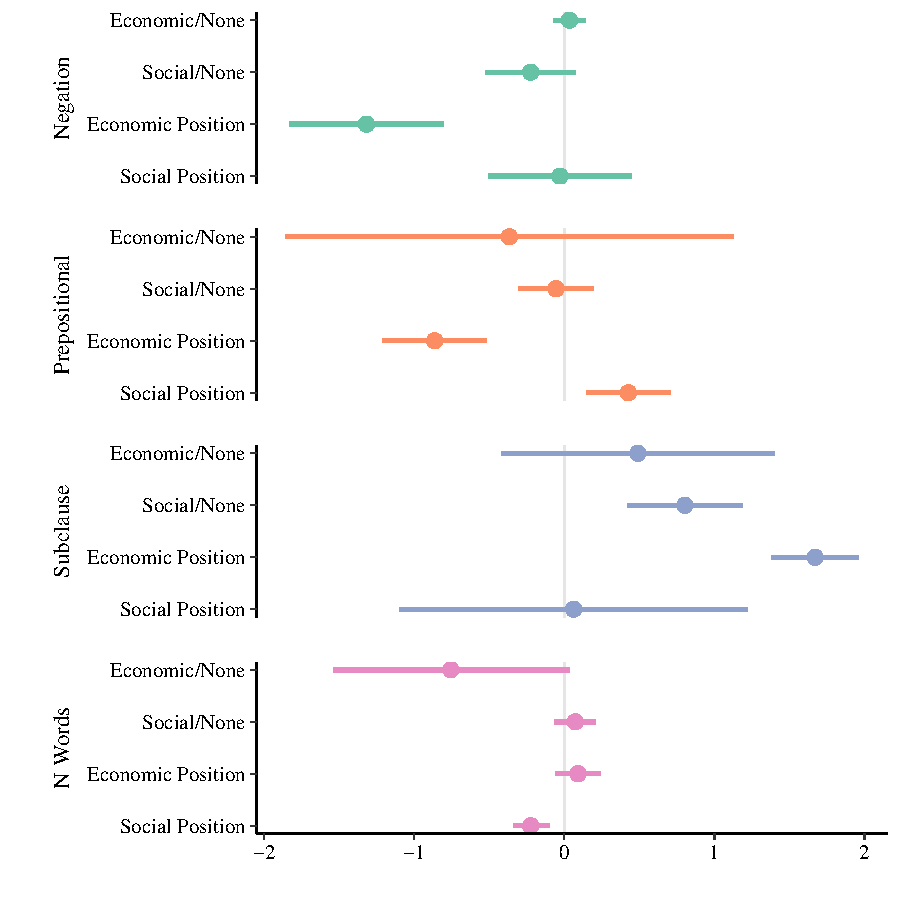
\includegraphics[width=0.8\linewidth]{beta_coefficients.pdf}
  \caption{Posterior mean and 95\% credible interval for $\bm\beta$ coefficients.}
  \label{fig:beta_coefficients}
\end{figure}

Whether a sentence contains a negation only has a significant effect on the discrimination for coding the economic scale. This effects is, however, quite large given the scale of the coefficients discussed above and negative. That is, sentences containing negation have a significantly lower discrimination which implies that the estimated latent coefficient for the sentence is less closely linked to the chosen code on the economic scale.
% What explains this?

In a similar vein, prepended prepositional phrases significantly decrease discrimination on the economic scale while there is no significant effect on choosing either the economic or social dimension. Interestingly, prepended prepositional phrases \emph{increase} the discrimination for assigning a position on the social scale. As this goes against the theory of misclassification we discuss above, this results warrants more investigation. A possible explanation might be that there are few cases of sentences coded as containing a social policy statement with negation. Also, results from \citet{Benoit2016} suggest that choosing a position on the social scale was generally associated with lower discrimination.
% Maybe we could explain this by looking at the number of

The results for the indicator for containing any subclause are puzzling given our theory. Deciding on whether a sentence contains a social policy statement and choosing a position on the economic scale seems to be significantly easier, on average, for sentences which contain a subclause than sentences without one. One potential explanation is that having a subclause is not a specific enough feature to reliably effect misclassification as about one in four sentences contains a subclause (see table~\ref{tab:summary-linguistic}).

Another possible explanation would be that it might be easier to assign codes to longer sentences, as they could contain additional information to base the judgement on. Sentences that contain a subclause tend to be longer than sentences that do not. However, the coefficient for the number of words associated with these two dimension is not significantly different from 0. The number of words in a sentence only has a significant effect on coding the position on the social scale. Here, longer sentences seem to be harder to code reliably. It is still possible that raw length of sentence does not capture the additional information added by short qualifying or clarifying subclauses.

\section{Discussion}
Although preliminary, our results indicate that linguistic features, such as negation and clause position, have some effect on how well humans differentiate between ideological positions. These results are not entirely novel in light of years of research in psycholinguistics and human perception of language stimuli. However, coupled with the fact that those features vary over time and can be associated with electoral victories and entering government, this paints a cautious picture of complete disregarding of language when assigning content coding tasks to humans. We suggest that language homogeneity has to be checked rather than assumed prior to the start of content analysis that relies on human coders. Another possibility that we investigate by using Bayesian hierarchical item response theory, is to explicitly model these assumptions in a single-step estimation procedure. The results also provide some insight into the success of automated techniques that rely on \enquote{bag-of-words} assumption. We theorise that a reason for their notable performance lies in the benefits that coarsening raw text brings. Although some information is indeed lost when word order is disregarded, in certain applications, especially those that rely on concepts that can be expected to be expressed in word frequencies, this loss is outweighed by removing ambiguity that is inherent to language.

\newpage
\singlespacing
\bibliographystyle{chicago}
\bibliography{bibliography.bib}

\end{document}
